%!TeX root=MemoriaTFG.tex

%Introduction to GPS: The Global Positioning System
%OGC® Geography Markup Language (GML) — Extended schemas and encoding rules

\chapter{Conceptos principales}
En esta sección se pretenden introducir los conceptos básicos referentes al tipo de información, 
herramientas y formatos de datos geográficos con los que se trabaja durante toda la propuesta.

\section{Sistemas de navegación por satélite}
Los \ac{GNSS} son mecanismos formados por una red de satélites utilizados 
para situar elementos en la superficie terrestre. Destacan los sistemas GALILEO, GLONASS y GPS,
de origen Europeo, Ruso y Americano respectivamente, siendo este último el que explicaremos 
con más detalle.
El Sistema de Posicionamiento Global, también llamado \ac{GPS} por sus siglas en inglés 
lo forma un mínimo de 24 satélites en órbita que proporcionan información de posicionamiento y tiempo 
accesible para cualquier usuario. El funcionamiento de estos sistemas se basan el cálculo de la 
distancia de un punto de la tierra a tres satélites aplicando conocimientos de "Position resection". \cite{Langley01}
Esta información tiene una precisión de 100 y 156 metros para la componente horizontal y vertical, 
respectivamente al 95$\%$ de probabilidad \cite{ElRabbany01}.

\subsection{GIS}
%Qué es un GIS
Los Sistemas de Información Geográfica, \ac{GIS},  son aplicaciones que permiten almacenar, manipular y presentar la información geográfica \cite{EPA01}.Entre el gran número de aplicaciones GIS destacan ArcGIS y QGIS, siendo la primera software no libre publicado por la empresa Esri y la segunda software libre por la Open Source Geospatial Foundation.
\begin{figure}[htb]
\begin{center}
\includegraphics[width=0.6\textwidth]{./Imagenes/ArcGIS.png}
\caption{Ejemplo de la aplicacion ArcGis}
\label{fig:ArcGis01}
\end{center}
\end{figure}
\begin{figure}[htb]
\begin{center}
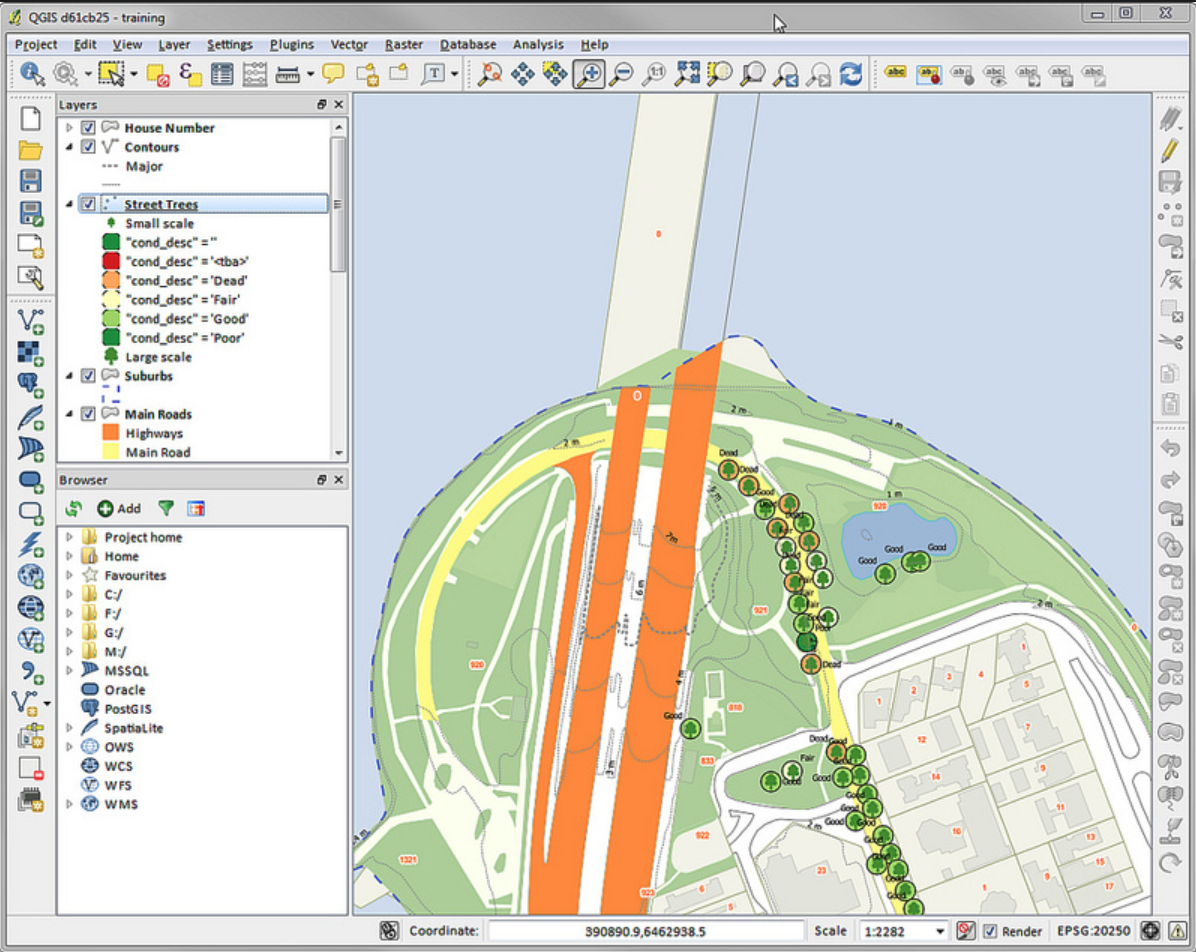
\includegraphics[width=0.6\textwidth]{./Imagenes/QGIS.png}
\caption{Ejemplo de la aplicacion QGIS}
\label{fig:QGIS01}
\end{center}
\end{figure}

\newpage
\subsection{Fuentes de datos}
Estas herramientas necesitan que los datos obtenidos por \ac{GPS}  sigan un formato compatible. 
Estas herramientas soportan una gran diversidad de formatos que se dividen en ráster y Vectoriales. 

\subsubsection{Formato ráster}
La respresentación de los datos se hace a partir de píxeles regulares de valor único.
La geofrafía de un espacio queda descrita en una matriz en la que cada cuadrícula 
almacena la información como altitud o superficie. Entre los formatos ráster más 
populares estan Esri Grid, GeoTIFF, JPEG2000 \cite{Morales01}.

\begin{figure}[htb]
\begin{center}
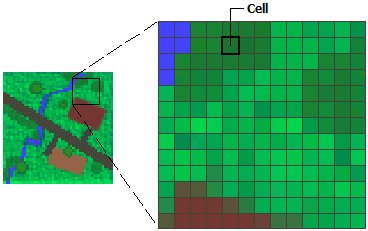
\includegraphics[width=0.6\textwidth]{./Imagenes/RasterImage.png}
\caption{Ejemplo de territorio en formato ráster. \cite{ArgGis01}}
\label{fig:PointGeneration02}
\end{center}
\end{figure}

\subsubsection{Formato vectorial}
los formatos vectoriales se basan en la representación mediante puntos, líneas y polígonos.
De este segundo grupo destacamos los siguientes:
\begin{description}
\item [\ac{GML}] Lenguaje procedente del esquema \ac{XML} que almacena información geográfica \cite{OGC01}.
\item[\ac{KML}] Lenguaje basado en el esquema \ac{XML} para la representar información 
geográfica en un navegador cartográfico como Google Earth o Google Maps \cite{OGC02}.%(KML 2.1 
\item[\ac{GPX}]Formato basado en el esquema \ac{XML} para el intercambio de datos \ac{GPS}. 
En especial para la descripción de points, tracks y routes. La principal ventaja  de este formato 
es la capacidad de intercambio de datos entre diferentes  programas en diferentes entornos 
(Windows, MacOS, Linux, Palm, PocketPC). Es este el formato seleccionado como entrada de datos 
\ac{GPS} del desarrollo de este proyecto \cite{Topografix01}.
\end{description}

\section{Estructura de los ficheros \ac{GPX}}
El formato \ac{GPX} al ser basado en \ac{XML} establece sus propias etiquetas y tipos con la información 
del fichero y del espacio geográfico que describe. La etiqueta principal gpx (gpxType) es la raíz del 
fichero \ac{XML}. Presenta de forma obligatoria la versión y el creador del fichero, así como una cabecera 
de metadatos, dónde se describe la información del fichero, autor, así como restricciones de copyright 
de ser necesario. Los elementos esenciales para la descripción de la información geográfica son los siguientes:
\begin{description}
\item[\textit{Waypoints} (wptType)] Representación de un punto de interés. Consta de una secuencia de elementos 
opcionales para añadir posición, descripción y precisión, así como los atributos obligatorios de latitud/longitud.
\item[\textit{Route} (rteType)] Lista ordenada de Waypoints.  Representan una sucesión de puntos hacia un destino. 
Contiene una secuencia de elementos descriptivos de carácter opcional.
\item[\textit{Tracks} (trkType)] Lista ordenada de puntos que escriben un camino. Contiene el mismo tipo de 
secuencia de elementos descriptivos de carácter opcional.
\end{description}

Podemos ver en la siguiente figura un ejemplo de  una ruta de una ruta de senderismo por la Serra de Tramuntana
de Mallorca.

\begin{figure}[htb]
\begin{center}
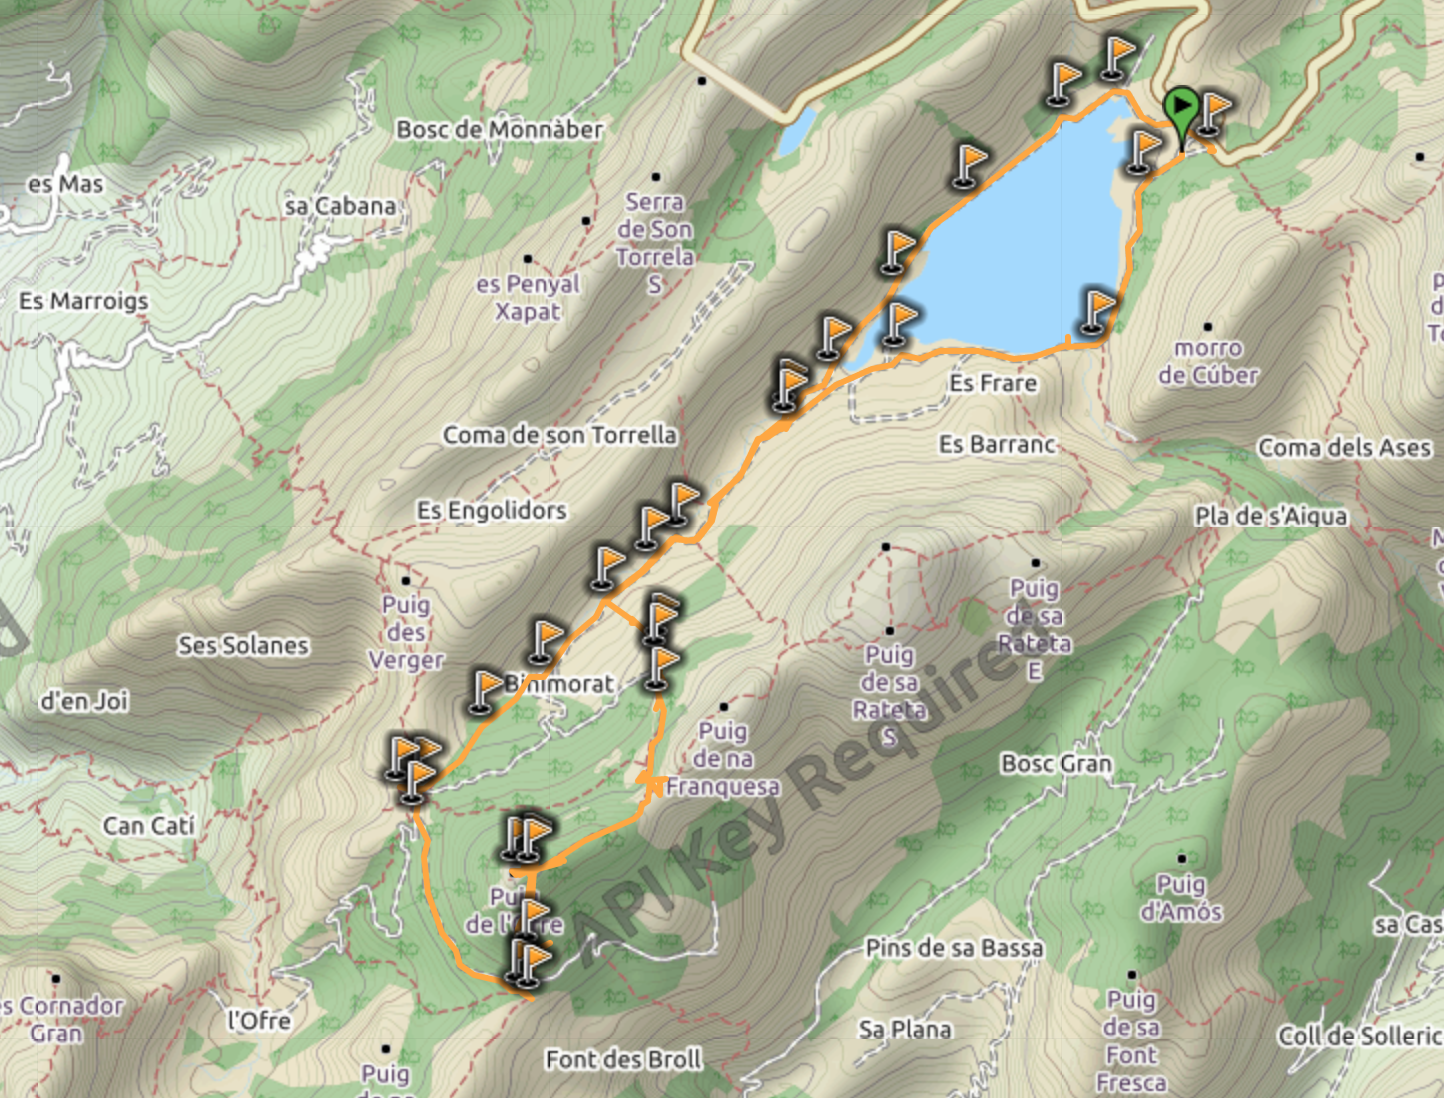
\includegraphics[width=0.6\textwidth]{./Imagenes/RutaOfre.png}
\caption{Ejemplo de Ruta del Puig de l'Ofre, Mallorca, Illes Balears, España.}
\label{fig:PointGeneration02}
\end{center}
\end{figure}

\begin{figure}[htb]
\begin{center}
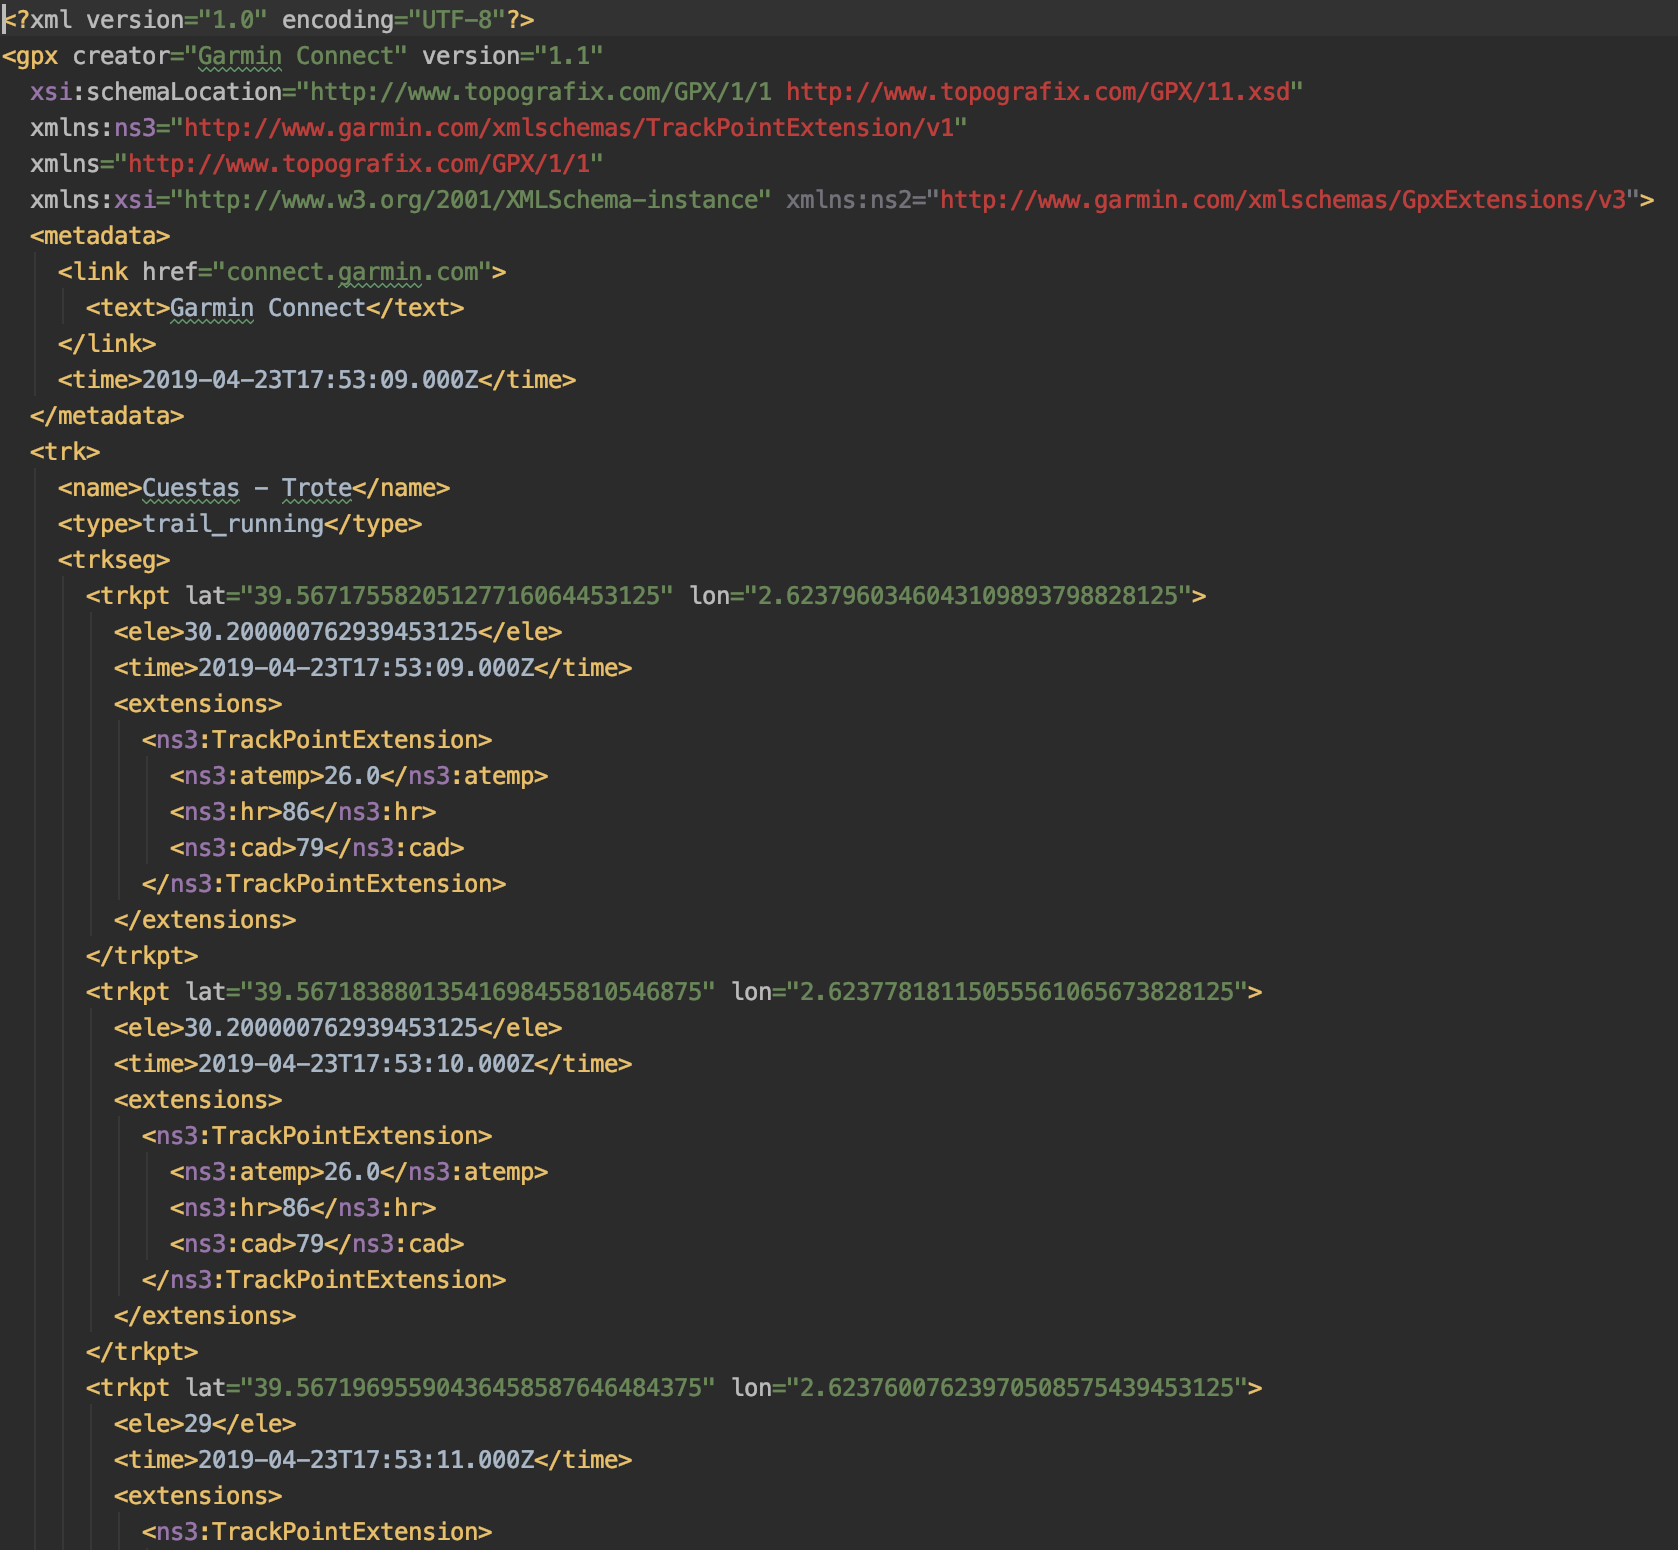
\includegraphics[width=0.75\textwidth]{./Imagenes/GPXExample.png}
\caption{Ejemplo de código de un fichero .\ac{GPX}}
\label{fig:PointGeneration02}
\end{center}
\end{figure}



\newpage

\section{Open Street Map}
%Qué es OSM. Aplicaciones
\ac{OSM} es un mapa interactivo open-source que permite visualizar información geográfica. Las gran ventaja 
de \ac{OSM} es la cantidad de herramientas aportadas por la comunidad que permiten importar, analizar, 
visualizar y editar la información. El formato de fichero \ac{GPX} es el más utilizado dentro de esta herramienta. 

\begin{figure}[htb]
\begin{center}
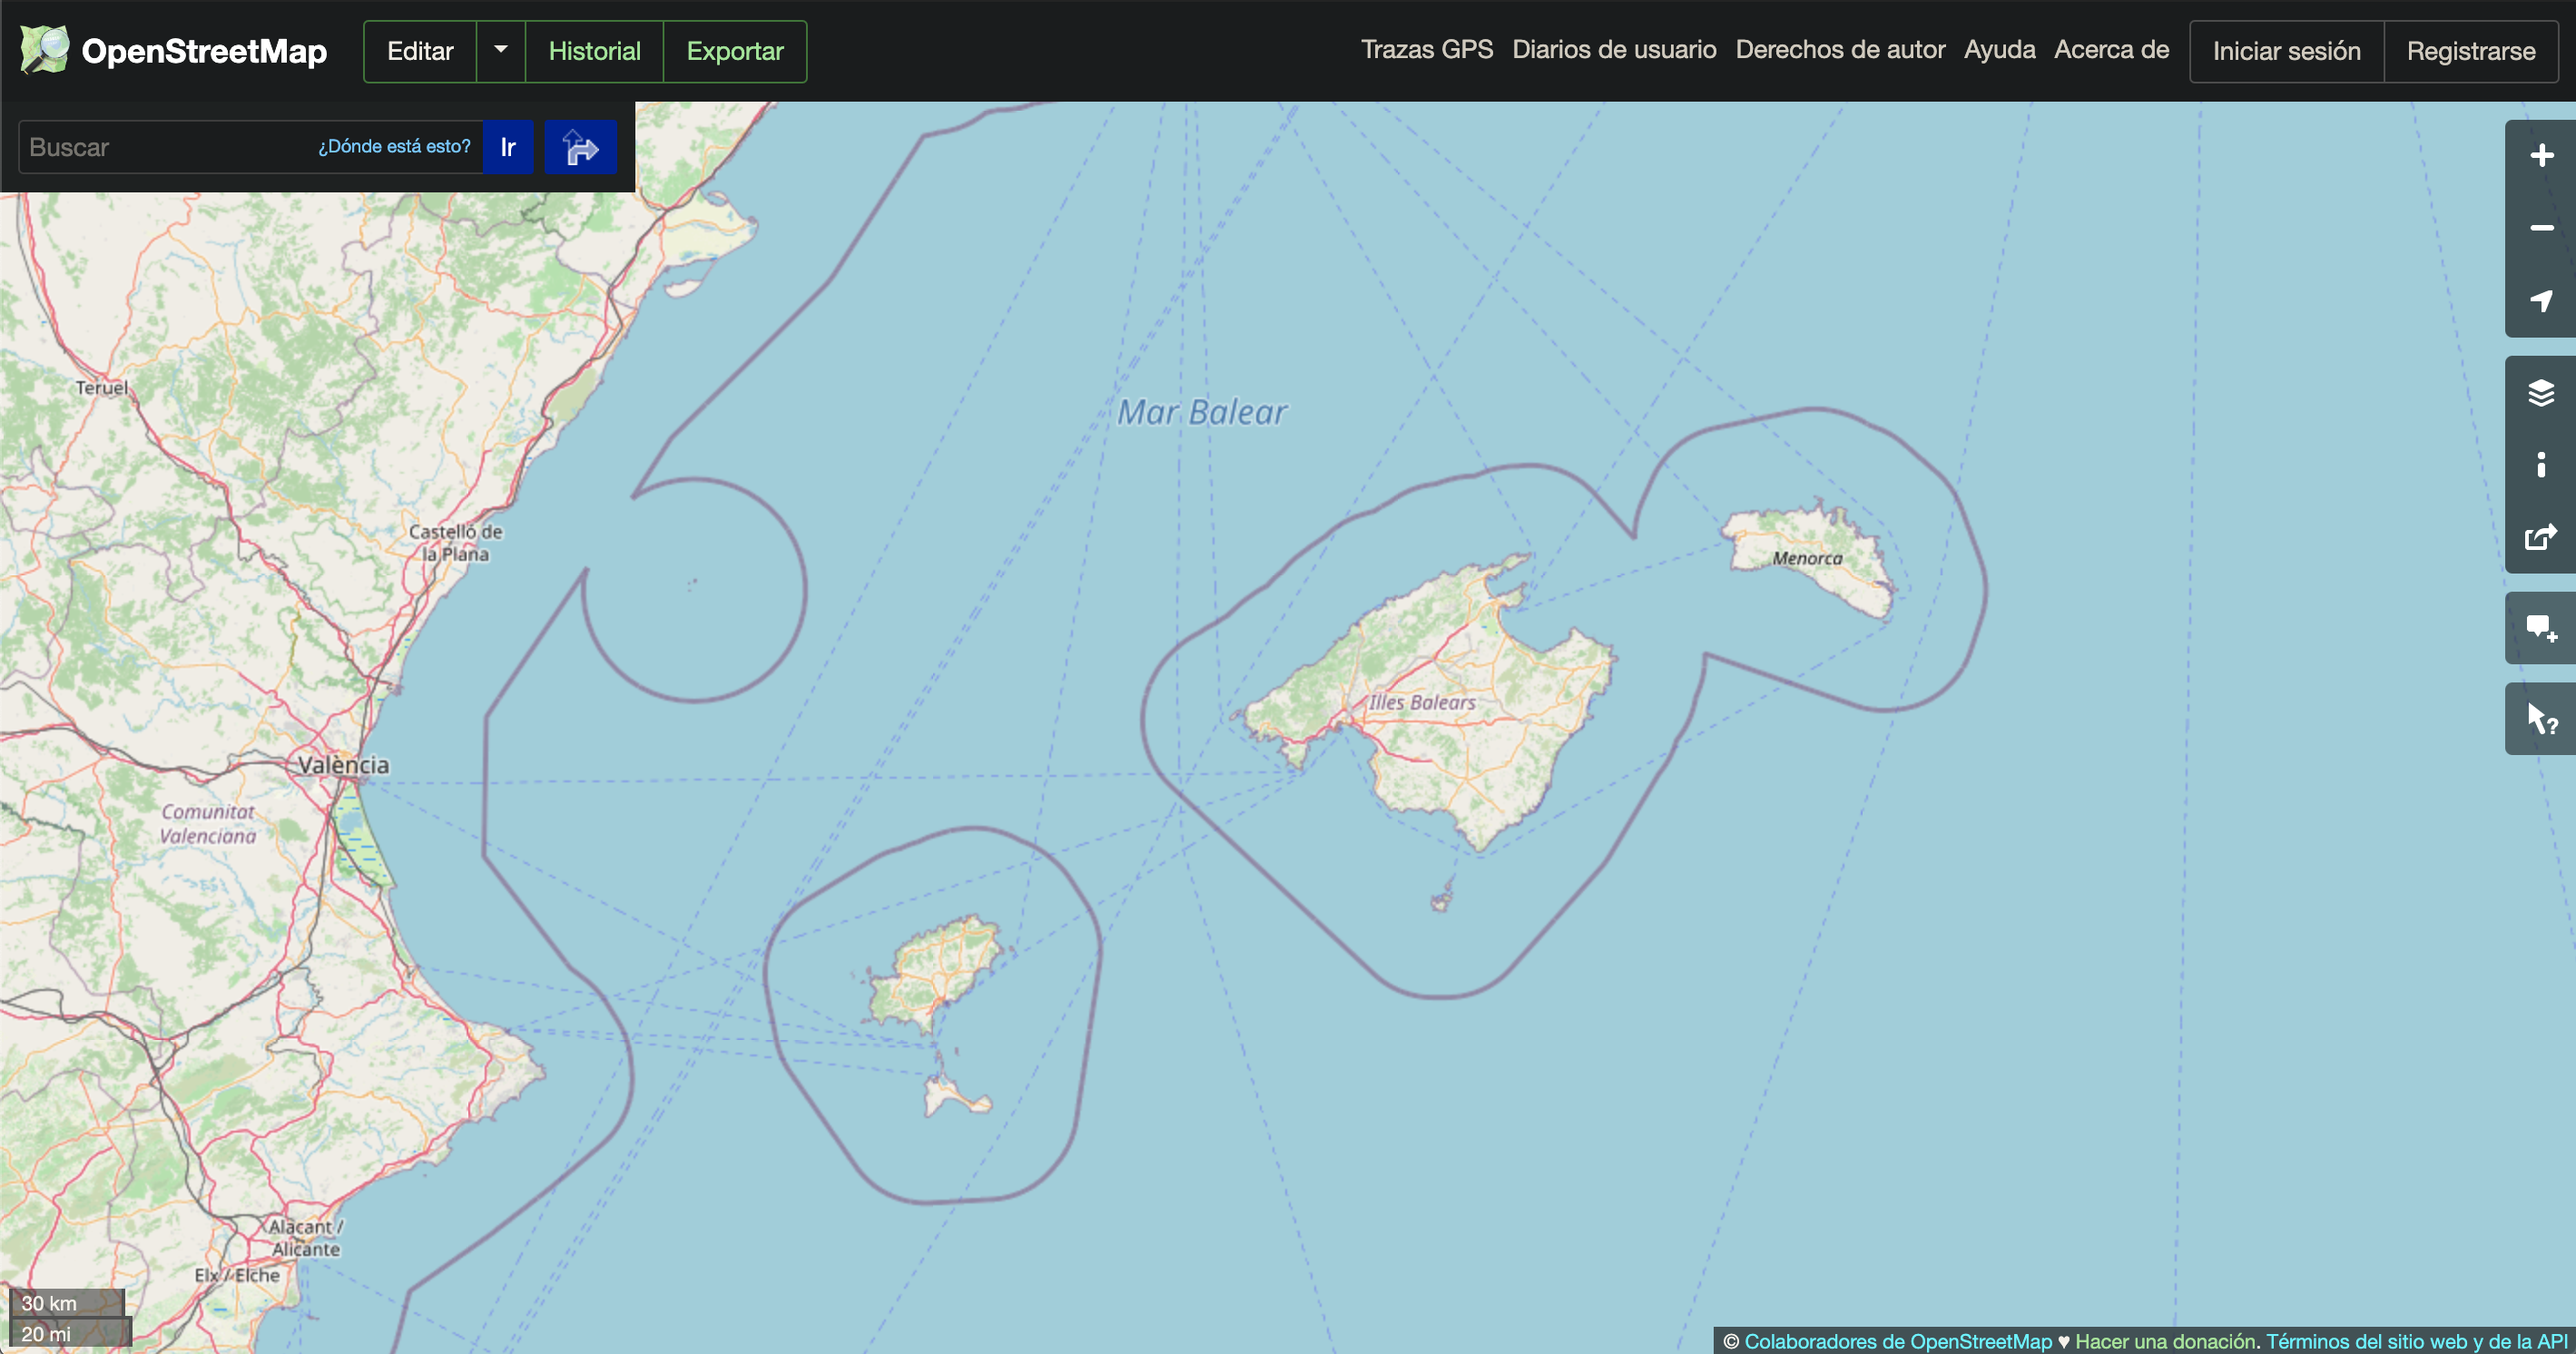
\includegraphics[width=0.9\textwidth]{./Imagenes/OSMExample.png}
\caption{Ejemplo de muestra de OSM de las Illes Balears, España.}
\label{OSMExample}
\end{center}
\end{figure}



